% ==============================================================
\chapter{Introduction}
% ==============================================================

The availability of genome sequences is a key prerequisite for modern 
biological research.
After the discovery of the DNA double helix structure \citep{Watson1953},
genome sequencing techniques have been developed and refined over the decades
\citep{Gilbert1973, Sanger1975}, 
culminating in the publication of the full human genome sequence in 2001 
\citep{Venter2001}.
Aside from the ambiguities introduced by non-coding regions in the genome 
\citep{Gilbert1978} and alternative splicing of genes \citep{Black2003}, 
the genome provides, in theory, all necessary information about which proteins 
can potentially be expressed in a cell.
However, in order to study the dynamic nature of a cell or organism, as for 
example in response to changing environmental conditions, the static information
provided by the genome is not sufficient. 
The transcriptome provides information about gene expression at the RNA level. 
DNA microarray techniques can be employed to screen the regulation of many
genes in parallel on the transcript level \citep{Schena1995}.

Complementing transcriptomics, the field of proteomics deals with the total
set of proteins expressed in a cell, tissue, or organism, at a defined time
point and under certain conditions \citep{Yarmush2002, Yates2009}.
In contrast to transcriptomics, proteomics is situated at the stage of 
translation and protein synthesis, and therefore most accurately reflects the 
phenotype of a cell. 
Mass spectrometry provides an excellent means for proteome analysis
\citep{Aebersold2003}, with speed, accuracy, and sensivity rapidly increasing
within the past two decades.
The major goals of mass spectrometry-based proteomics are protein 
identification and quantitation.
However, since most proteins are too heavy to be measured directly, the
analysis is usually performed on the peptide level, with proteins being digested
prior to the measurement using proteolytic enzymes such as Trypsin, Lys-C, or 
Pepsin. 
The inherent ambiguity introduced by protein isoforms or alternative splicing
poses an additional challenge when peptide identifications are shifted to
the protein level.
In addition to the raw amino acid sequence encoded by a gene, post-translational
modifications play an important role in defining the actual function of a
protein.
Post-translational modifications may modify a protein by adding an enzyme or by
chemically modifying certain residues.
Furthermore, structural adjustments such as the formation of disulfide 
bonds between Cysteine residues may be required for the protein to become 
functional.
Employing mass spectrometry, it is possible not only to identify peptides and
proteins, but also to study their various modifications.
Another application of mass spectrometry-based analysis is the localization of
proteins to certain compartments of a cell, for example by semi-quantitative
analysis.

Although modern mass spectrometers are very sensitive, a couple of sample 
preparation steps must be carried out in order to achieve comprehensive 
proteome coverage. 
An example of a mass spectrometry-based proteomics workflow for peptide 
and protein identification is depicted in Fig.~\ref{fig:proteomics-overview}.

\begin{figure}
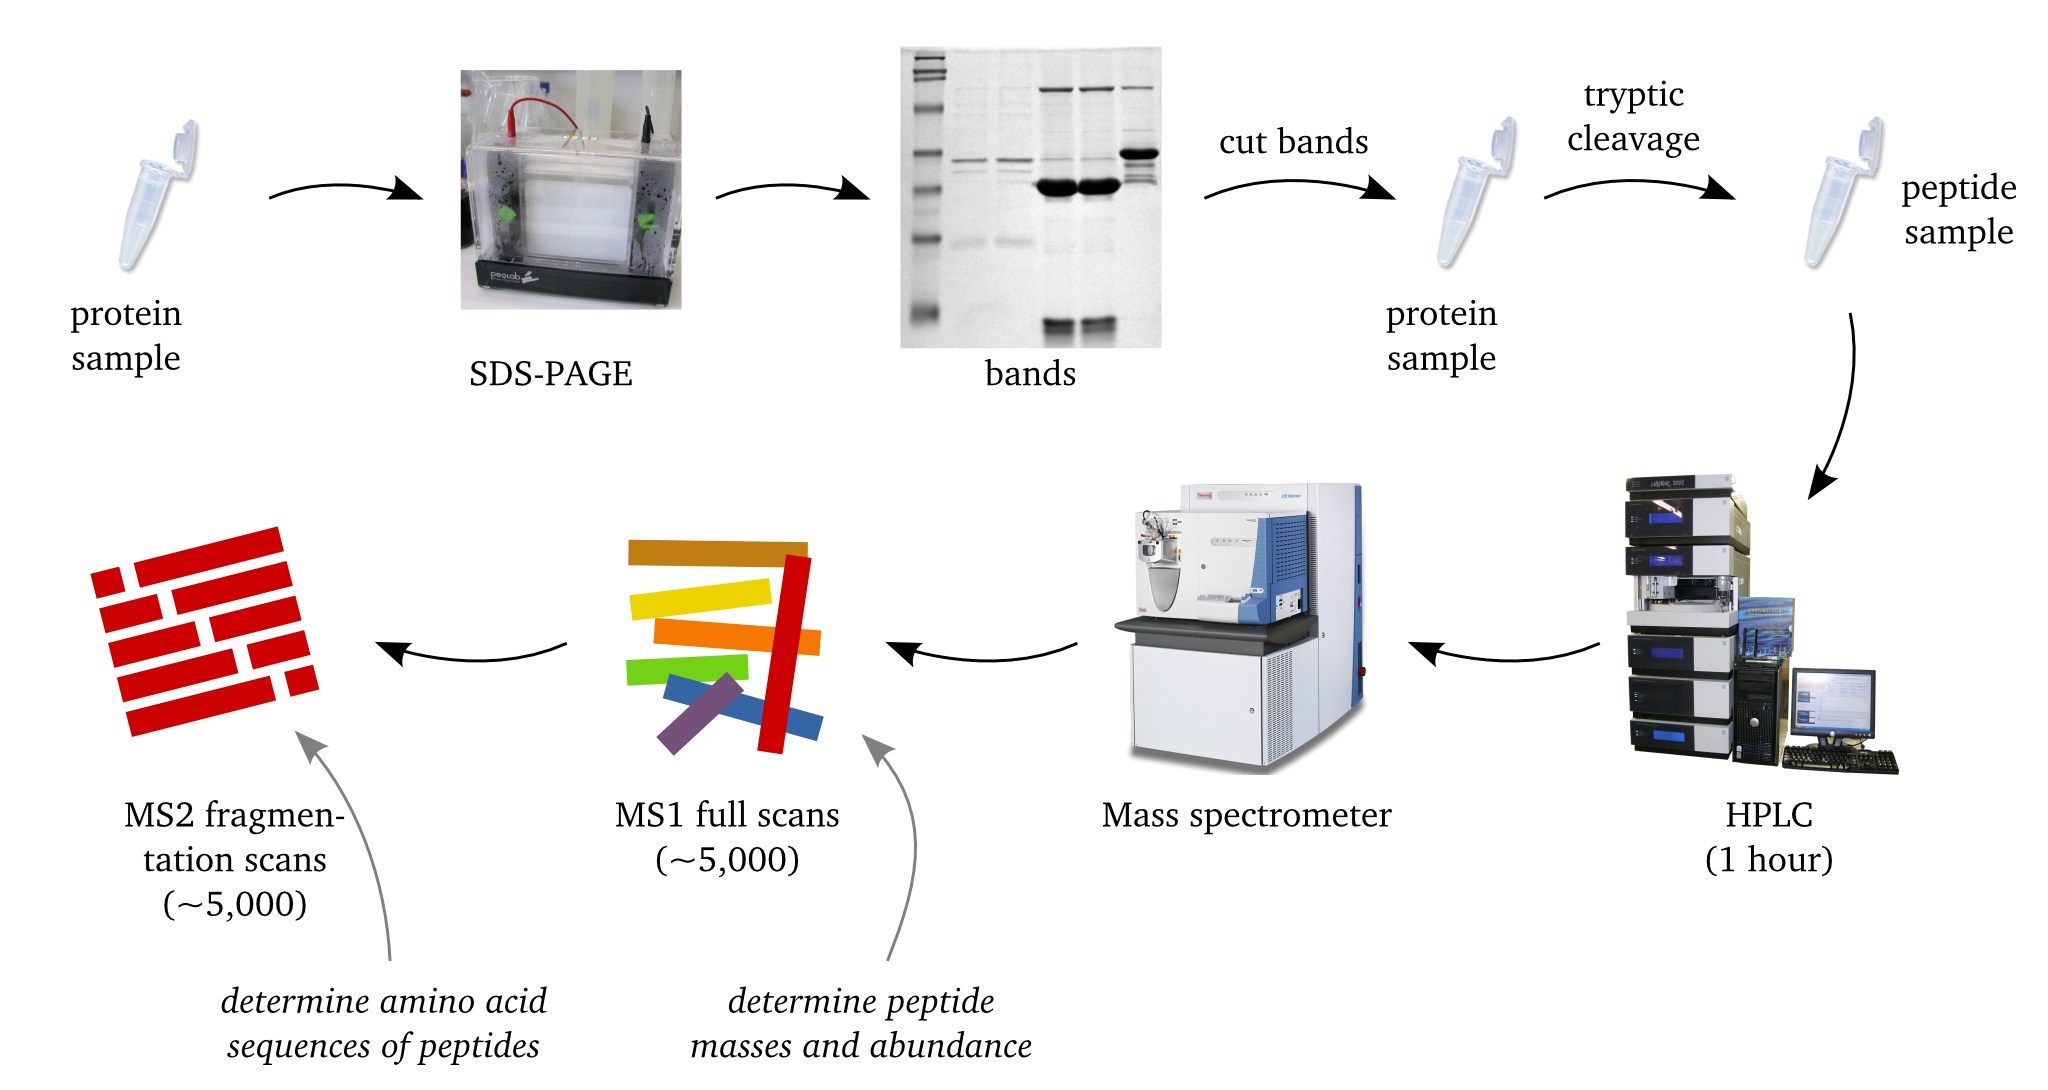
\includegraphics[width=\textwidth]{figures/Proteomics.jpg}
\caption{
{\bf Example of a mass spectrometry-based proteomics experiment workflow.} 
Protein samples are fractionated via SDS-PAGE and resulting bands are excised and
digested proteolytically. In order to further separate the complex mixture, 
the resulting peptides are loaded onto a HPLC column and subsequently eluted 
and injected into the mass spectrometer. Full scans and fragmentation scans
are recorded as peptide elution is in progress for a pre-defined amount of time.
}
\label{fig:proteomics-overview}
\end{figure}

% --------------------------------------------------------------
\section{Acquisition of mass spectrometric data}
% --------------------------------------------------------------

In the following, the steps involved in the acquisition of mass spectrometric
data are described.

\subsection{Preprocessing of biological samples}

Although mass spectrometric analysis of intact proteins has been successfully
reported \citep{Lee2002, Taylor2003}, such an approach is not feasible in 
general because the high mass of proteins cannot be accounted for with most
types of mass spectrometers.
In addition, low abundant proteins may be missed in complex samples due to
the fact that there are many more highly abundant proteins present.
To overcome these obstacles, a couple of sample preprocessing steps are usually
undertaken, with possible variations depending on the experimental context.

\subsubsection{Gel electrophoresis}

Due to the high dynamic range of protein expression levels, complex protein 
mixtures tend to produce less comprehensive results because low abundant 
proteins are `shadowed' by highly abundant proteins. 
Gel electrophoresis may be used as a first sample separation step in which
proteins are ordered by size, resulting in a number of fractions which can
be analyzed individually.
For SDS-PAGE, a sodium dodecyl sulfate polyacrylamide gel is prepared and
proteins are loaded into wells in the gel.
An electric field is applied to the gel, thus inducing an electromotive force 
on the proteins which move through the gel at a speed which depends on their
size and charge.
However, SDS leads to denaturation of proteins and results in an overall
negative charge for all proteins. 
Thus, the protein migration speed is only dependent on the size of the protein.
Individual spots of equally-sized proteins may be visualized using ethidium 
bromide, silver, or Coomassie dye and subsequently excised.

In order to achieve even higher sample separation, two-dimensional gel 
electrophoresis may be used \citep{Klose1975, O'Farrell1975}.
Here, proteins are additionally separated by a second physicochemical property
such as their isoelectric point.
As in the SDS-PAGE approach, resulting spots may be excised and subjected 
to mass spectrometric analysis.

\subsubsection{Proteolysis}

In order to break proteins up into small, mass spectrometry-compatible peptides, 
proteolytic enzymes are used.
Among the various choices of possible enzymes, Trypsin has become very popular
because it results in short peptides with a basic residue at the C-terminus
\citep{Olsen2004}.
Trypsin cleaves specifically at the C-terminal side of Lysine and Arginine 
residues, given that no Proline residue is located at the other side of the 
cleavage site.
Alternative enzymes such as Asp-N and Glu-C are sometimes used to generate
complementing peptides which overlap with the tryptic peptides in order to 
increase sequence coverage of peptide identifications \citep{Steen2004}.
Although Trypsin, Asp-N and Glu-C are very sequence-specific, the possibility 
of missed cleavage sites must be taken into account during data analysis.

\subsubsection{Liquid chromatography}

HPLC, SCX, IEF

\subsection{Ionization of molecules}

\begin{todo}
ESI, MALDI
\end{todo}

\subsection{Mass analysis}

\begin{todo}
TOF, IT, Orbitrap
\end{todo}

\subsection{Mass spectra}

\begin{todo}
data formats (DTA, MGF, mzData, mzXML, mzML)
\end{todo}

\subsubsection{Full scans (MS)}

\begin{todo}
precursor peaks
\end{todo}

\begin{figure}[h]
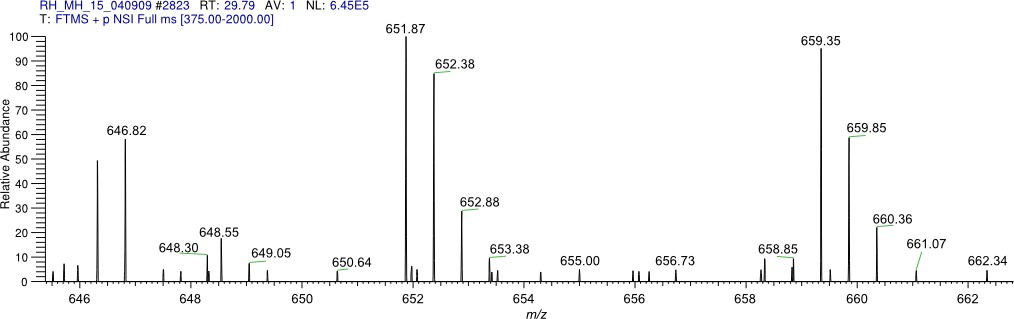
\includegraphics[width=\textwidth]{figures/ms1-scan.jpg}
\caption{
{\bf Example of a full scan.} 
Caption here.
}
\label{fig:full-scan}
\end{figure}

\subsubsection{Fragmentation scans (MS/MS)}

\begin{todo}
CID, a/b/c/x/y/z ions
\end{todo}

\begin{figure}[h]
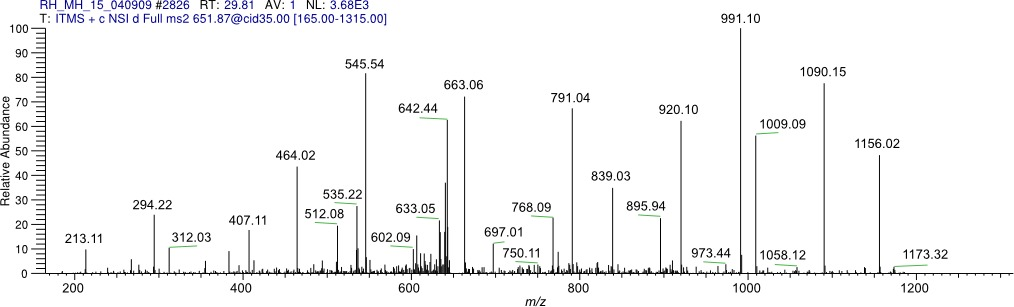
\includegraphics[width=\textwidth]{figures/ms2-scan.jpg}
\caption{
{\bf Example of a fragmentation scan.} 
Caption here.
}
\label{fig:fragmentation-scan}
\end{figure}

\begin{figure}[h]
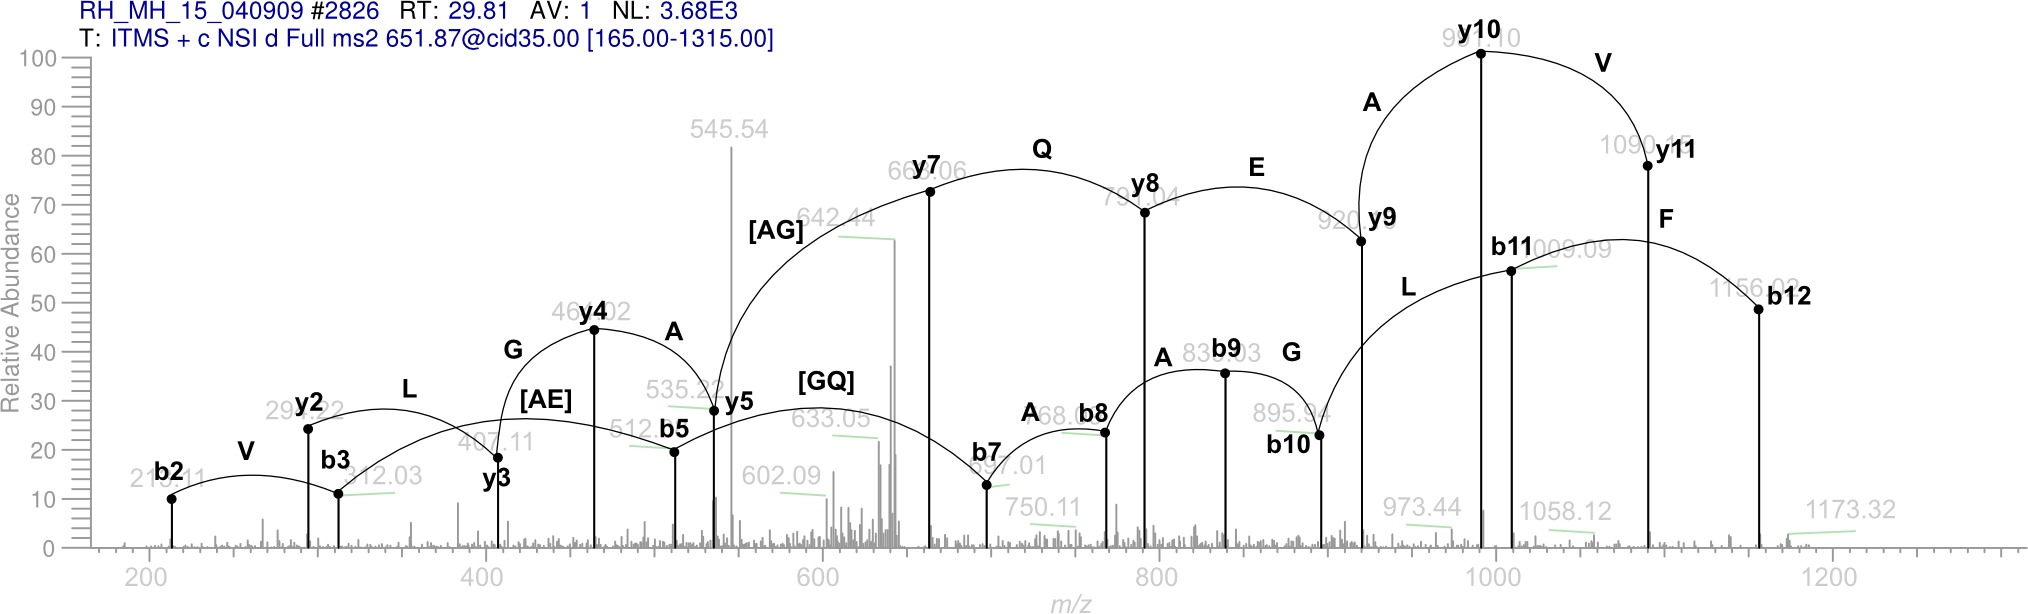
\includegraphics[width=\textwidth]{figures/ms2-scan-b-y-1.jpg}
\caption{
{\bf Fragmentation scan with b and y ion series mass ladders superimposed.} 
Caption here.
}
\label{fig:fragmentation-scan-b-y}
\end{figure}


% --------------------------------------------------------------
\section{Data evaluation}
% --------------------------------------------------------------

\subsection{Sequence databases}

\subsubsection{Genome sequences}

\begin{todo}
genome sequencing
180+ genomes sequences [Yates2009]
\end{todo}

\subsubsection{Protein databases}

\begin{todo}
genome annotation
\end{todo}

\subsection{Identification}

\subsubsection{Peptide mass fingerprinting}

\begin{todo}
sets of proteotypic precursor masses
\end{todo}

\subsubsection{Database search}

\begin{todo}
in silico digestion and matching via cross correlation or OMSSA-type & whatnot
\end{todo}

\subsubsection{De novo sequencing}

\begin{todo}
unbiased sequences, quite ambiguous, GPF by Jens Allmer
\end{todo}

\subsection{Quantitation}

\subsubsection{Chemical labeling}
 
\begin{todo}
ICAT, iTRAQ
\end{todo}

\subsubsection{Metabolic labeling}

\begin{todo}
SILAC, 15N
\end{todo}

\subsubsection{Label-free quantitation}

\begin{todo}
across several runs
\end{todo}

% --------------------------------------------------------------
\section{Proteogenomics}
% --------------------------------------------------------------

\begin{todo}
genome annotation/gene model prediction, AUGUSTUS, external hints, 
EGASP, exon splice graph, GPF
\end{todo}

% --------------------------------------------------------------
\section{Chlamydomonas reinhardtii}
% --------------------------------------------------------------

\begin{todo}
soil or freshwater green alga, unicellular, hetertroph / photoautotrop, sexual & asexual
\end{todo}

\subsection{Anaerobic metabolism}

\begin{todo}
hydrogen production
\end{todo}

% --------------------------------------------------------------
\section{Thalassiosira oceanica}
% --------------------------------------------------------------

\begin{todo}
deep water diatom
\end{todo}

\subsection{Iron deficiency}

\begin{todo}
hydrogen production
\end{todo}
